%! TEX PROGRAM = pdflatex
\documentclass[a4paper]{article}

\usepackage[utf8]{inputenc}
\usepackage{microtype, listings, amsmath, amssymb, csquotes}
\allowdisplaybreaks
\usepackage{tikz}
\usepackage{pgfplots}
\usepackage{subcaption}
\usepackage{xparse}
\usepackage{graphicx}
\usepackage{bm}
\usepackage{amsthm}
%\usepackage{subfig}

\usepackage{alphalph}
\usepackage[hidelinks]{hyperref}
\usepackage{cleveref}
\usepackage[margin=1in]{geometry}

\usepackage[style=numeric,sorting=none]{biblatex}
\addbibresource{main.bib}

\hypersetup{
    colorlinks=true,
    linkcolor=red,
    citecolor=green,
    filecolor=magenta,
    urlcolor=cyan
}


\newenvironment{psmallmatrix}
  {\left(\begin{smallmatrix}}
  {\end{smallmatrix}\right)}

\newcommand{\wrt}{w.r.t.}
\DeclareMathOperator*{\argmax}{arg\,max}
\DeclareMathOperator*{\argmin}{arg\,min}

\newtheorem{theorem}{Theorem}[section]
\newtheorem{corollary}{Corollary}[theorem]
\newtheorem{lemma}[theorem]{Lemma}
\newtheorem{definition}{Definition}

\let\emptyset\varnothing

%was node [circle,draw=black,inner sep=0pt,minimum size={width("AAA")}] {\AlphAlph{\x}\AlphAlph{\y}};}}
% was [square,draw=black]
\tikzset{square/.style={rectangle,inner sep=0pt,minimum size=1cm}}
\providecommand{\toroid}[1]{
    \draw[shift={(-0.5,0.5)}] (1,-1) grid (#1+1,-#1-1);
        \foreach \x in {1,...,#1} {
            \foreach \y in {1,...,#1} {
                \node at (\x,-\y) {\AlphAlph{\y}\AlphAlph{\x}};}}
}
\providecommand{\superToroid}[4]{
    \IfBooleanTF#1{\providecommand{\shading}{white}}{\providecommand{\shading}{gray}}
    \draw[shift={(-0.5,0.5)}] (1,-1) grid (#2+1,-#2-1);
        \foreach \x in {1,...,#2} {
            \foreach \y in {1,...,#2} {
        \pgfmathtruncatemacro{\xpos}{(\x-1)*#2+(\y-1)}
        \pgfmathtruncatemacro{\ypos}{((#4-1)*#2+(#3-1))}
        \ifnum\xpos<\ypos
        \providecommand{\param}{white}
        \else
        \providecommand{\param}{\shading}
        \fi
\node[square,draw=black,fill=\param] at (\x,-\y)[align=center] {\AlphAlph{#4}\AlphAlph{#3}\\ \AlphAlph{\y}\AlphAlph{\x}};}}
}
\providecommand{\toroidWarp}[1]{
    \scalebox{0.8}{
    \begin{tikzpicture}
        \toroid{#1}
        \foreach \x in {1,...,#1} {
            \node at (\x,0) {\AlphAlph{#1}\AlphAlph{\x}};
            \node at (\x,-#1-1) {\AlphAlph{#1}\AlphAlph{\x}};
        }
        \foreach \y in {1,...,#1} {
            \node at (0,-\y) {\AlphAlph{\y}\AlphAlph{#1}};
            \node at (#1+1,-\y) {\AlphAlph{\y}\AlphAlph{1}};
        }
    \end{tikzpicture}
}}

\providecommand{\toroidAxes}[4]{
    \superToroid{#1}{#2}{#3}{#4}
        \foreach \x in {1,...,#2} {
            \node at (\x,0) {\AlphAlph{\x}};
        }
        \foreach \y in {1,...,#2} {
            \node at (0,-\y) {\AlphAlph{\y}};
        }
}

\NewDocumentCommand{\nestedToroid}{sm}{
    \scalebox{0.8}{
    \begin{tikzpicture}[scale=#2+1]
        \begin{scope}[scale=1]
            \draw[shift={(-0.5,0.5)}] (1,-1) grid (#2+1,-#2-1);
            \foreach \x in {1,...,#2} {
                \node at (\x,-0.25) {\AlphAlph{\x}};
            }
            \foreach \y in {1,...,#2} {
                \node at (0.25,-\y) {\AlphAlph{\y}};
            }
            \foreach \xa in {1,...,#2} {
                \foreach \ya in {1,...,#2} {
                    \begin{scope}[shift={({\xa-0.5+1/(#2+1)^2},{-\ya+0.5-1/(#2+1)^2})},scale={1/(#2+1)}]
                        \toroidAxes{#1}{#2}{\xa}{\ya}
                    \end{scope}
                }
            }
        \end{scope}
    \end{tikzpicture}
    }
}
%a
\NewDocumentCommand{\twodcomparison}{sm}{
    \IfBooleanTF#1{\providecommand{\shading}{white}}{\providecommand{\shading}{gray}}
    \scalebox{0.8}{
\begin{tikzpicture}
        %\draw[shift={(-0.5,0.5)}] (0,0) grid ({(#2^2)},{-(#2^2)});
        \foreach \x in {1,...,#2} {
            \foreach \xa in {1,...,#2} {
                \node at ({(\x-1)*#2+(\xa-1)},1) {\AlphAlph{\x}\AlphAlph{\xa}};
        }}
        \foreach \y in {1,...,#2} {
            \foreach \ya in {1,...,#2} {
                \node at (-1,{-((\y-1)*#2+(\ya-1))}) {\AlphAlph{\y}\AlphAlph{\ya}};
        }}
        \foreach \xa in {1,...,#2} {
            \foreach \ya in {1,...,#2} {
            \foreach \xb in {1,...,#2} {
                \foreach \yb in {1,...,#2} {
                \pgfmathtruncatemacro{\xpos}{(\xa-1)*#2+(\ya-1)}
                \pgfmathtruncatemacro{\ypos}{((\xb-1)*#2+(\yb-1))}
                %\pgfmathtruncatemacro\xpos{}
                %\pgfmathtruncatemacro\ypos{}
        \ifnum\xpos<\ypos
        \providecommand{\param}{white}
        \else
        \providecommand{\param}{\shading}
        \fi
\node[square,draw=black,fill=\param] at (\xpos,-\ypos)[align=center] {\AlphAlph{\xb}\AlphAlph{\yb}\\ \AlphAlph{\xa}\AlphAlph{\ya}};}}
            }
        }
\end{tikzpicture}
}}

\newcommand{\drawGrid}[2]{
    %1 is the length of the raw toroid
    %2 is the list
    \begin{tikzpicture}
    \foreach \token [count=\i from 0] in #2 {
        \pgfmathtruncatemacro{\x}{mod(\i,#1)}
        \pgfmathtruncatemacro{\y}{\i/#1}
    \node[square,draw=black] at (\x,-\y) {\token};}
    \end{tikzpicture}
}
\ExplSyntaxOn
\NewDocumentCommand{\superposition}{mm}{
    \scalebox{0.8}{
\begin{tikzpicture}
        %\draw[shift={(-0.5,0.5)}] (0,0) grid ({(#2^2)},{-(#2^2)});
        \foreach \x in {1,...,#1} {
            \foreach \xa in {1,...,#1} {
                \node at ({(\x-1)*#1+(\xa-1)},1) {\AlphAlph{\x}\AlphAlph{\xa}};
        }}
        \foreach \y in {1,...,#1} {
            \foreach \ya in {1,...,#1} {
                \node at (-1,{-((\y-1)*#1+(\ya-1))}) {\AlphAlph{\y}\AlphAlph{\ya}};
        }}
        \foreach \xa in {1,...,#1} {
            \foreach \ya in {1,...,#1} {
            \foreach \xb in {1,...,#1} {
                \foreach \yb in {1,...,#1} {
                \pgfmathtruncatemacro{\xpos}{(\xa-1)*#1+(\ya-1)}
                \pgfmathtruncatemacro{\ypos}{((\xb-1)*#1+(\yb-1))}
            \str_if_eq:eeTF {\AlphAlph{\xb}\AlphAlph{\yb}} {\clist_item:nn {#2}{(\xa-1)*#1+\ya}}
            {\providecommand{\param}{gray}}
            {\providecommand{\param}{white}}
\node[square,draw=black,fill=\param] at (\xpos,-\ypos)[align=center] {\AlphAlph{\xb}\AlphAlph{\yb}\\ \AlphAlph{\xa}\AlphAlph{\ya}};}}
            }
        }
\end{tikzpicture}
}}
\ExplSyntaxOff

\title{\emph{Reversing Nearness} via Gradient Descent}
\author{Jason Ken A}

\begin{document}
\maketitle
\tableofcontents

\section{Introduction}%
\label{sec:introduction}

Gradient descent is an iterative algorithm to optimize\footnote{usually in the context of minimization, hence `descent'} a continuous function. It does so by shifting parameters in the direction of opposite of their gradient with respect to (\wrt{}) the function, that is:
\begin{align*}
         \theta'=\theta-\alpha \frac{d}{d\theta}L(\theta).
\end{align*}
Here, $\theta$ is the parameter to optimize,to minimize the value of function $L$, and $\alpha$ is an arbitrary scaling factor usually called \emph{learning rate}. Gradient descent can be generalized to multi-variable optimization through the use of partial derivatives within Jacobian matrices. Regardless, it self-evident why  continuous functions are required.

The primary goal of this essay is to measure the generalization capability of gradient descent, whether a discrete loss function can be generalized to a continuous loss, and therefore whether optimum discrete parameters can be obtained. ``Reversing Nearness'', a programming contest held by Al Zimmermann, proved to be a suitable testbed for this purpose, because traditionally, it had been approached with non-gradient optimization methods, such as hill climbing and simulated annealing, all of which are beyond the scope of this essay. To the best of my knowledge, a gradient based approach has never been attempted on the competition, for good reason: it is a discrete optimization problem. The objective is deceptively simple, given a grid of tokens, ``your task is to rearrange the tokens so that pairs of tokens that are near each other become far from each other and those that are far from each other become near.''\cite{zimmermann} The definitions of ``token'', ``grid'', and distance will be explained within the essay.

``It will be fun'', I said, after all, are they not the reason for my calculus classes? Hence, my research question: \emph{Is gradient descent a viable approach for \emph{Reversing Nearness}?}

\begin{enumerate}
  \item \textbf{Short answer:} Yes
  \item \textbf{Long answer:}
\end{enumerate}

\section{Problem Statement}%
\label{sec:problem_statement}

\subsection{Toroidal Graph}%
\label{sub:toroidal_graph}


According to \href{http://azspcs.com/Contest/Nearness}{AZSPCS}, a toroidal graph is defined as an $N\times N$ grid of unique tokens -- here presented as $IJ$, where $I$ and $J$ represent the alphabetic indices (eg. $A$ corresponds to 1) of the rows and columns respectively -- whose edges wrap around. For $N=4$, the grid is shown in \autoref{fig:toroidExample}. The tokens outside of the square grid represent tokens which ``wrap around'' the grid (hence the toroidal grid).
\begin{figure}[htpb]
    \centering
    \toroidWarp{4}
    \caption{A $4\times 4$ toroidal grid}%
    \label{fig:toroidExample}
\end{figure}

\subsection{Evaluation Function}%
\label{sub:evaluation_function}

The goal of the challenge (and hence this essay) is to create a new grid -- with tokens from the original grid to be arranged in any order -- which minimizes a loss function (which quantifies failure) defined as follows:
\begin{enumerate}
    \item For each pair of tokens, calculate the squared distance between them in the new grid,
\item multiply it with its squared distance within the original grid
\item The sum of these multiplications is the value of the loss
\end{enumerate}
As is with all loss functions, the goal is to minimize the loss function.

\subsubsection{Distance Metric}%
\label{ssub:distance_metric}
If 2 two-dimensional coordinates are defined as $s_1=(x_1,y_1)$ and $s_2=(x_2,y_2)$, the Euclidean distance $d$ is defined as

\begin{equation}
    \label{eq:euclid}
    d(s_1,s_2)=\sqrt{(x_2-x_1)^2+(y_2-y_1)^2}=\sqrt{(\Delta x)^2+(\Delta y)^2}
\end{equation}

and the squared Euclidean distance $d^2$ evaluates to
\begin{equation}
    d^2(s_1,s_2)=(\Delta x)^2+(\Delta y)^2
    \label{eq:squaredEuclid}
\end{equation}
simplifying much of the computation.

But with a toroidal surface, both $\Delta x$ and $\Delta y$ have 2 possible values. A one-dimensional case with toroidal surface of length $N$ is shown in \autoref{fig:2distanceexample}. These two distances can be written as
\begin{align*}
    %\label{eq:naiveToroidDistance}
    \Delta_1(x)&=x_2-x_1 \\
    \Delta_2(x)&=(x_1-0)+(N-x_2)=x_1+N-x_2
\end{align*}

\begin{figure}[tpb]
    \centering
    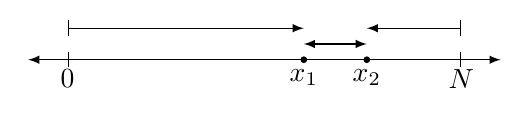
\begin{tikzpicture}
        \draw[latex-latex] (-3,0) -- (3,0);
        \draw[|-|] (-2.5,0) node[below] {$0$} -- (2.5,0) node[below] {$N$};
        %\draw[|-|] (-2.5,-0.5) -- node[below] {$N$} (2.5,-0.5);
        \filldraw (0.5,0) circle (1pt) node[below] {$x_1$};
        \filldraw (1.3,0) circle (1pt) node[below] {$x_2$};
        \draw[latex-latex] (0.5,0.2) -- (1.3,0.2);
        \draw[latex-|] (1.3,0.4) -- (2.5,0.4);
        \draw[|-latex] (-2.5,0.4) -- (0.5,0.4);
    \end{tikzpicture}
    \caption{One-dimensional diagram of toroidal distance}%
    \label{fig:2distanceexample}
\end{figure}


To obtain a general equation which works with both $x_1>x_2$ and $x_1<x_2$, we can write
\begin{align*}
    \Delta_1(x)&=\lvert x_2-x_1 \rvert \\
    \Delta_2(x)&=\min{(x_1,x_2)}+N-\max{(x_1,x_2)}
    %\label{eq:absoluteToroidDistance}
\end{align*}
where $\lvert a\rvert$ is the absolute value of $a$, $\min{(a,b)}$ and $\max{(a,b)}$ are defined as the minimum and maximum of $a$ and $b$ respectively. $\min$ and $\max$ are used to determine the  ``left-most'' and the ``right-most'' numbers.

Since, the distance can only have 1 value, it is defined as
\begin{align*}
    \Delta x=\min{(\Delta_1(x),\Delta_2(x))}
\end{align*}

Generalizing it to 2 dimensions, we get
\begin{align*}
    d(s_1,s_2)&=\sqrt{(\Delta x)^2+(\Delta y)^2} \\
    d^2(s_1,s_2)&=(\Delta x)^2+(\Delta y)^2
\end{align*}
where $d^2$ is the distance metric to be used in our calculations.

\subsubsection{Token Comparisons}%
\label{ssub:token_comparisons}
To be able to perform comparisons for every possible pair of tokens, a grid of comparisons (between two tokens to obtain distances) is required. A viable approach would be to to represent the comparison in a 4-dimensional grid (or tensor), where for every token in the toroidal grid, we compare it to every token. An example of the structure of the comparison for a $2\times 2$ grid is shown in \autoref{fig:4dcomparison}. The white boxes denote duplicate comparisons (eg. $
\begin{smallmatrix}
    BA\\ AA
\end{smallmatrix}
$ is identical to
$
\begin{smallmatrix}
    AA\\ BA
\end{smallmatrix}
$), because the distance is invariant to the order of the tokens.


But since removing the irregularly shaped duplicate entries will be a hassle, we can simplify the problem by reducing the dimensionality of the grid: from a 4-dimensional grid $A_{ijkl}$ into a 2-dimensional grid $A_{ij,kl}$. An example is shown in \autoref{fig:2dcomparison}. By doing so, we can easily remove the duplicate entries by multiplying it with the upper triangular matrix, see \autoref{ssub:loss_function_as_matrix_multiplications}. Let $C(X)$ denote a function mapping, returning this comparison grid for an input toroidal grid $X$. Note that if $X$ is a grid of the form $N\times N$, $C(X)$ has the form $N^2\times N^2$

\begin{figure}[htpb]
    \centering
    \label{fig:twodcomparisonGrid}
\end{figure}

\begin{figure}[htpb]
    \centering
    \begin{subfigure}[t]{0.5\textwidth}
    \begin{center}
    \nestedToroid{2}
    \end{center}
    \caption{$A_{ijkl}$, a 4-dimensional comparison}
    \label{fig:4dcomparison}
    \end{subfigure}%
    ~
    \begin{subfigure}[t]{0.5\textwidth}
    \begin{center}
    \twodcomparison{2}
    \end{center}
    \caption{$A_{ij,kl}$ a 2-dimensional comparison}
    \label{fig:2dcomparison}
    \end{subfigure}

    \caption{Tensors $C$ representing comparison grids of a $2\times 2$ toroidal grid, where every element represents the toroidal distance between $T_{ij}$ and $T_{kl}$, where $T$ is the toroidal grid. Shaded cells denote unique comparisons.}%
    \label{fig:comparisonGrids}
\end{figure}

\subsubsection{Loss Function as Matrix Multiplications}%
\label{ssub:loss_function_as_matrix_multiplications}
Let $\odot$ denote the element-wise matrix multiplication, and $O$ denotes the original grid. The loss function for toroidal grid $X$ is equal to
\begin{equation}
    L(x)=\sum C(X)\odot C(O)\odot U
\end{equation}
where $C(X),C(O),U$ are matrices of the form $N^2\times N^2$, and $U_{ij}$ is defined with the piece-wise defined function:
\begin{equation}
    U_{ij}=
    \begin{cases}
        1, & j\geq i \\
        0, & j<i
    \end{cases}
\end{equation}
an example the matrix U with shape $4\times 4$ is as follows:
 \begin{equation}
    \begin{pmatrix}
        1&1&1&1\\
        0&1&1&1\\
        0&0&1&1\\
        0&0&0&1
    \end{pmatrix}
\end{equation}


\section{Superposition}%
\label{sec:superposition}
Since the entries into the toroidal grid are discrete (ie. discrete matrix indices correspond to discrete coordinates within the grid), it is not yet possible to optimize the loss function. Therefore, relaxing the constraints to enable ``superposition'' --- here defined as having a token being in multiple positions, with each of its positions having its own ``probabilities'' --- is essential. In this essay, ``probability'' will not refer to the likeliness of a random event, but rather, the confidence of a token in its posiiton. Let $S$ denote the superposition grid.
\begin{figure}[htpb]
    \centering
    \begin{subfigure}[t]{0.5\textwidth}
    \begin{center}
    \nestedToroid*{2}
    \end{center}
    \caption{$A_{ijkl}$, a 4-dimensional superposition}
    \end{subfigure}%
    ~
    \begin{subfigure}[t]{0.5\textwidth}
    \begin{center}
    \twodcomparison*{2}
    \end{center}
    \caption{$A_{ij,kl}$ a 2-dimensional superposition}
    \end{subfigure}

    \caption{Tensors $S$ representing superpositions of a $2\times 2$ toroidal grid, where every element $S_{ijkl}$ represents the probability of the token $KL$ being in the of position $IJ$ in the original grid}%
    \label{fig:superposition}
\end{figure}

A simple method of allowing superposition, is by allowing any token to be in any position, which again, can be visualized as a 4-dimensional matrix, and 2-dimensional matrix, as seen in \autoref{fig:superposition}, and again, to reduce complexity we choose the 2-dimensional model. But this time, in contrast to \autoref{fig:comparisonGrids}, the elements of the grid \emph{do not represent comparisons}, but rather, the element $S_{i,j,k,l}$ (in the case of a 4-dimensional superposition) or $S_{ij,kl}$ (in the case of a 2-dimensional superposition), represent the probability of the token $\bm{KL}$ inhabiting the position of the token $\bm{IJ}$ \emph{within the original grid $O$}. Further constraints to enforce the concept of probabilities will be discussed in \autoref{sub:constraints}. Note that now the rows represents various positions within the grid $O$, and the columns represents the possible token values. An example is shown in \autoref{fig:superpositionExample}.


\begin{figure}[htpb]
    \centering
    \begin{subfigure}[t]{0.5\textwidth}
    \begin{center}
\drawGrid{2}{{BB,AB,BA,AA}}
    \end{center}
    \caption{$A_{ijkl}$, an example toroidal grid}
    \end{subfigure}%
    ~
    \begin{subfigure}[t]{0.5\textwidth}
    \begin{center}
\superposition{2}{BB,AB,BA,AA}
    \end{center}
    \caption{$A_{ij,kl}$ superposition of the grid on the left}
    \end{subfigure}

    \caption{Shaded cells represent cells with probability 1, the rest have probability 0}
    \label{fig:superpositionExample}
\end{figure}

\subsubsection{Generalization of the Loss Function}%
\label{ssub:generalization_of_the_loss_function}

Defining the loss function for this formulation requires us to compare \emph{every} value within \emph{every} position, to \emph{every other} value within \emph{every} position.\footnote{The wording is important} this is  And we must do so, while taking both of their confidence's into account (ie. the distance metric should be scaled by their confidence). Therefore, the distance should be scaled with
\begin{equation}
    S_{ab}S_{cd}
\end{equation}

The distance between these two probabilities is defined as $C_{a,c}$, because only the indices $a$ and $c$ correspond to positions on the grid (thus being important in calculating distance), whereas $b$ and $d$ correspond to only the token itself.

Alike with the situation in \autoref{ssub:token_comparisons}, we must prevent duplicate comparisons between values (not position), for example: each of %
[$\begin{smallmatrix}AA\\AA\end{smallmatrix}$,%
$\begin{smallmatrix}AB\\AA\end{smallmatrix}$,%
$\begin{smallmatrix}BA\\AA\end{smallmatrix}$,%
$\begin{smallmatrix}BB\\AA\end{smallmatrix}$] should be compared to
[$\begin{smallmatrix}AA\\AB\end{smallmatrix}$,%
$\begin{smallmatrix}AB\\AB\end{smallmatrix}$,%
$\begin{smallmatrix}BA\\AB\end{smallmatrix}$,%
$\begin{smallmatrix}BB\\AB\end{smallmatrix}$], but not vice versa, because the values (not the positions) will have been compared already. Again, to do so, we must construct an upper triangular matrix $U$, of the shape $N^2\times N^2$.

Therefore, the loss function can be written as
\begin{equation}
    L(X)=\sum_{a}^{N^2} \sum_{b}^{N^2} \sum_{c}^{N^2} \sum_{d}^{N^2} S_{a,b} S_{c,d} C_{a,c}C_{b,d}U_{a,c}
\end{equation}

\begin{itemize}
    \item [$\sum_{a}^{N^2}$] Represents an iteration over Source Positions
    \item [$\sum_{b}^{N^2}$] Represents an iteration over Source Values
    \item [$\sum_{c}^{N^2}$] Represents an iteration over Target Positions
    \item [$\sum_{d}^{N^2}$] Represents an iteration over Target Values
    \item [$S_{a,b}$] Represents the Probability of the Source Position and Value
    \item [$S_{c,d}$] Represents the Probability of the Target Position and Value
    \item [$C_{a,c}$] Represents the Distance between Source and Target Position
    \item [$C_{b,d}$] Represents the Distance between the Source and Target Values in the original grid
    \item [$U_{a,c}$] Upper triangular matrix to remove redundant value comparisons
\end{itemize}

\section{Optimization}%
\label{sec:optimization}

\subsection{Constraints}%
\label{sub:constraints}
To be able to properly model probability, the sum of the probabilities of each token in all of its positions must be equal to one. Similarly, the sum of the probabilities of each position, in all of its values must be equal to one. Therefore, the sums of each of the rows and each of the columns must be equal to one, this is called a Doubly Stochastic Matrix. To be able to enforce this constraint, the Sinkhorn-Knopp algorithm was developed.

\subsubsection{Sinkhorn-Knopp Algorithm}%
\label{ssub:sinkhorn_knopp_algorithm}

Given $K$ an $n\times n$ non-negative matrix, by repetitively normalizing the rows and columns, a doubly stochastic matrix can be obtained. A single iteration can be seen through the following equation

\begin{equation}
        K'=\left(\sum^N_i K_{ij}\right)^{-1}K\left(\sum^N_j K_{ij}\right)^{-1}
\end{equation}

\subsubsection{Non-negative Matrices}%
\label{ssub:non_negative_matrices}
Since Sinkhorn-Knopp requires a non-negative matrix, and because negative probabilities make no sense, at every iteration of Sinkhorn-Knopp and Gradient Descent, the values have to be maintained above $0$.
\begin{equation}
        K'_{ij}=\max(K_{ij},0)
\end{equation}

\subsection{Gradient Descent}%
\label{sub:gradient_descent}
Gradient Descent is an algorithm to iteratively optimize a convex function, with knowledge of the derivative of the function with respect to all of the function parameters $\theta$. In the case of optimizing a loss function, steps must be taken in the direction opposite to the gradient, therefore, the equation is as follows
\begin{equation}
         \theta'=\theta-\alpha \frac{\delta}{\delta \theta}L(\theta)
\end{equation}
where $\alpha$ is a parameter determining how big of a change there is between iterations of gradient descent.

\subsubsection{Derivative of Loss Function coming Soon}%
\label{ssub:derivative_of_loss_function_coming_soon}



%\section{Discretization}%
\label{sec:discretization}
Recall that our end goal is not to optimize the continuous representation of the toroidal grid, $S$, but rather the discrete grid $X$. To be able to convert $S$ into $X$, we must take into account the tokens in the positions with the highest confidence. And once this token is established within $X$, all of the entries within $S$ within the same token value (ie. same row), or same position (ie. same column) should be removed. This should be repeated until all the entries within $X$ are filled.

Let $r$ and $c$ (representing rows and columns) be empty sets. The procedure is then as following.
\begin{align*}
    r,c\leftarrow r,c\cup \argmax_{m\notin r,n\notin c}S_{m,n}\\
    X_{i,j}=O_{k,l}
\end{align*}
while $\argmax$ is defined. The conversion from $m$ and $n$ to $i,j$ and $k,l$ is stated within \ref{ssub:token_comparisons}.

\subsection{A Comprehensive Example}%
\label{sub:a_comprehensive_example}



\section{Evaluation}%
\label{sec:evaluation}
\subsection{Graphs of Loss over Time}%
\label{sub:graphs_of_loss_over_time}

\subsection{Comparison to State of the Art Lower Bounds}%
\label{sub:comparison_to_state_of_the_art_lower_bounds}

\subsection{Limitations of Computational Complexity}%
\label{sub:limitations_of_computational_complexity}

\subsection{Limitations of How to Discretive Superpositions}%
\label{sub:limitations_of_how_to_discretize_superpositions}

\subsection{Summary}%
\label{sub:summary}



\section{Acknowledgements}%
\label{sec:acknowledgements}

I would like to thank Emmerich Education Center for kindly providing computational resources used within this Extended Essay.


\printbibliography
\end{document}
